\documentclass[11pt,twocolumn]{article}
\usepackage{abstract}
\usepackage{geometry}
\geometry{verbose,tmargin=3cm,bmargin=3cm,lmargin=2.5cm,rmargin=2.5cm}
\usepackage[utf8]{inputenc}
\usepackage{graphicx}
\usepackage{listings}
\lstset{
    escapeinside={(*}{*)}
}

\usepackage{hyperref}
\lstset{aboveskip=24pt,belowskip=24pt}
\usepackage{mathtools}
\usepackage{amsfonts}
\usepackage{amsmath}
\lstset{language=Python}
\usepackage[english]{babel}
\usepackage[numbers]{natbib}
\usepackage{titlesec}
\usepackage{subcaption}
\usepackage{float}
\usepackage[strings]{underscore}
\usepackage{etoolbox}
\apptocmd{\sloppy}{\hbadness 10000\relax}{}{}

\newcommand{\floor}[1]{\left\lfloor #1 \right\rfloor}
\newcommand{\ceil}[1]{\left\lceil #1 \right\rceil}

\newcommand{\dd}[1]{\mathrm{d}#1}
\setlength{\columnsep}{0.75cm}

\newcommand*\ttvar[1]{\texttt{\expandafter\dottvar\detokenize{#1}\relax}}
\newcommand*\dottvar[1]{\ifx\relax#1\else
  \expandafter\ifx\string.#1\string.\allowbreak\else#1\fi
  \expandafter\dottvar\fi}
\usepackage{xurl}

% abstract styling
\renewenvironment{abstract}%
{%
  \centerline%
  {\large\bf Abstract}%
  \begin{quote}%
}
{
  \par%
  \end{quote}%
  \vskip 1ex%
}

\hypersetup{
    colorlinks=true,
    linkcolor=black,
    filecolor=black,
    citecolor=black,
    urlcolor=blue,
}


\title{Comparison of phylogenetic reconstruction methods}
\author{Lívia Qian\\KTH Royal Institute of Technology\\School of Electrical Engineering and Computer Science\\liviaq@kth.se}

\begin{document}

\twocolumn[
  \begin{@twocolumnfalse}
	\date{}
	\maketitle

	\begin{abstract}
The aim of this paper is to briefly describe and compare the performance of some widely accepted and one lesser-known method for phylogenetic reconstruction. Instead of trying to be a comprehensive guide summarizing the theoretical background of phylogenetics, it focuses on the main principles of creating simple phylogenetic trees and the conclusions I reached while testing these methods. While my primary goal was not to optimize them and making them scale to more complex data, approximating the time complexity of each algorithm was a crucial part of the experiments besides measuring the accuracy of the generated trees.
    \end{abstract}
  \end{@twocolumnfalse}
]

\section{Introduction}

Phylogenetics is the study of the evolutionary history of species and groups of species. There are multiple forms of expressing the relationship between different groups; one common method is the construction of a phylogenetic tree (or evolutionary tree), a diagram containing all the taxa in the form of leaves. Common traits can be observed using DNA sequences or morphology, the latter being generally more complex due to the many characteristics I certain species can have. Phylogenetic trees can be rooted and unrooted; the former is a version representing not only the similarity between each taxon but the ancestral relationships as well, while the latter form only illustrates the connection between the taxonomical units.

\section{Methods}

There are multiple steps involved in the construction of a phylogenetic tree. First, DNA sequences need to be of the same length, therefore a proper sequence alignment is needed. Regarding tree-creating algorithms, there are two main categories to choose from \cite{DeBruyn2013}: there are distance-based methods, which measure the differences between pairs of sequences and character-based methods, which use the columns of a sequence alignment directly. Examples of distance-based algorithms are neighbor joining (NJ) \cite{1987}, UPGMA \cite{sokal58}, WPGMA \cite{sokal58}, BIONJ \cite{Gascuel1997}, among others; the two most widely used character-based methods are the maximum parsimony (MP) and maximum likelihood (ML) methods. While all these techniques are popular, distance methods are usually recommended when computational time is an important factor; in other cases, parsimony and likelihood are preferred as they are more rigorous and have the ability to explore different combinations.

\subsection{Sequence alignment}

DNA (deoxyribonucleic acid) is a molecule that has two polynucleotide chains forming a double helix and carries information about an organism's development and reproduction. Genomes — genetic materials that make up an organism's body — consist of both protein-coding DNA (genomes) and non-coding DNA. DNA sequencing is the process of determining the order of nucleoids in the DNA; there are four bases — adenine, guanine, cytosine, and thymine — represented by characters A, G, C, T, whose order needs to be determined in order to gain relevant information about the molecule at hand. Sequence alignment is a way of arranging multiple DNA sequences into a matrix so that similar regions are grouped together — that is, regions that show a high degree of similarity in multiple sequences are placed underneath each other. As this process makes the characters in the sequences shift, a special character (commonly a "-") is used to fill in the gaps.

\subsection{Neighbor joining}

Neighbor joining is a distance-based method created by Saitou and Sei in 1987 \cite{1987}. A distance matrix is needed for all of the calculations in this method; this matrix should contain the pairwise distances between the input sequences according to a predefined distance metric. This matrix reduces in size after each step because of the clustering nature of the method.

In each iteration, the following steps are repeated until there are only two nodes left:

\begin{enumerate}
\item Calculate the divergence ($r$) for every element. Divergence for element $a$ is the sum of the distances from $a$ to all the other elements.

\item Calculate the new, alternative distance matrix using the following formula:
\begin{align}
d_{new}(i, j) = d(i, j) - \frac{r(i) + r(j)}{N - 2}
\end{align}
where $N$ is the number of elements in the current iteration.

\item Let's take the smallest value in the new distance matrix and the units belonging to it (let them be denoted by $a$ and $b$). Let's call their ancestral node $p$. The length of the new branches can be calculated as
\begin{align}
\delta(a, p) = \frac{d(a, b)}{2} + \frac{r(a) - r(b)}{2 (N - 2)} \\
\delta(b, p) = d(a, b) - \delta(a, p)
\end{align}

\item The rows and columns belonging to $p$ need to be added to the original distance matrix, while the ones belonging to $a$ and $b$ need to be deleted. After this, the difference between $p$ and the remaining nodes need to be calculated. Let's take an arbitrary element $c$ as an example:

\begin{align}
d(c, p) = \frac{d(a, c) + d(b, c) - d(a, b)}{2}
\end{align}

Branches $(a, p)$ and $(b, p)$ are now part of the tree that is being built.

\end{enumerate}

After this, we can join the remaining two elements by taking the ancestral node created in the last iteration and making the other node its child with their distance — that was specified in the last iteration — as the branch length.

Although it was originally intended for unrooted trees, NJ can easily be extended to rooted trees. This is one of the simplest and fastest methods in phylogeny, but it may not produce accurate results.

\subsection{WPGMA}

Originally attributed to Sokal and Michener \cite{sokal58}, WPGMA (weighted pair group method with arithmetic mean) is a hierarchical clustering method that uses a distance matrix in a similar fashion as the neighbor joining method. Each step consists of the following:

\begin{enumerate}
\item Find the smallest element in the distance matrix. Let's say that it is $d(a, b)$ and that it belongs to elements $a$ and $b$ (both of them can be clusters). Let's create a parent node called $p$.

\item We need to calculate branch lengths $\delta(a, p)$ and $\delta(b, p)$. If both $a$ and $b$ are leaves, these lengths are simply
\begin{align}
\delta(a, p) = \delta(b, p) = \frac{d(a, b)}{2}
\end{align}

If $a$ or $b$ are clusters, the height of the subtree belonging to them needs to be deducted from the amount mentioned before. Let's assume that $a$ is a cluster and that $c$ is a leaf of the subtree belonging to it. Then
\begin{align}
\delta(c, p) = \frac{d(a, b)}{2}
\end{align}
\begin{align}
\begin{split}
\delta(a, p) = \delta(c, p) - \delta(c, a) = \\
= \frac{d(a, b)}{2} - \delta(c, a)
\end{split}
\end{align}

In the case where $a$ is a leaf, $c$ could be represented by $a$ itself and $\delta(c, a)$ would be zero, therefore this is a generalized formula that can be used in any situation.

\item After cluster $p = (a, b)$ is created, it should be integrated into the distance matrix as a new element, therefore both a new column and a new row should be created (additionally, the columns and rows belonging to $a$ and $b$ can be deleted). Let's take an arbitrary element $q$. The distance between $q$ and $p$ can be calculated as
\begin{align}
d(p, q) = d((a, b), q) = \frac{d(a, q) + d(b, q)}{2}
\end{align}

\end{enumerate}

This is repeated until there is only one node left (the third step is not needed in the last iteration).

\subsection{UPGMA}

Also created by Sokal and Michener, UPGMA (unweighted pair group method with arithmetic mean) is highly similar to WPGMA. The only difference lies in that it keeps track of the number of elements in each cluster, making the resulting calculations unweighted. In Step 3, UPGMA uses cluster weights, resulting in the following distance matrix update rule:

\begin{align}
d((a, b), q) = \frac{d(a, q) \cdot m + d(b, q) \cdot n}{m + n}
\end{align}

where $a$ consists of $m$ and $b$ consists of $n$ elements. This is called \textit{proportional averaging}.

There are situations in which it is not recommended to use UPGMA, e.g., when the three-point criterion is not fulfilled. This criterion demands that for any three taxa $d(a, c) \le max(d(a, b), d(b, c))$, i.e., that the two greatest distances be equal. This is needed because UPGMA assumes a constant rate of evolution across lineages, therefore none of the leaves can be further away from the root than the others.

\subsection{Maximum parsimony}

Maximum parsimony is an umbrella term for all the methods that are based on the principle that a model is better than another if it implies fewer evolutionary events. The number of evolutionary events is represented by a cost called the \textit{parsimonious score}. There are two major categories: \textit{exact} methods are the ones that consider the score of all possible trees, thus giving a global minimum, and \textit{heuristic} methods are those that use some kind of technique to find a significant subset of all the trees and produces a somewhat sub-optimal result. As exact methods are often computationally infeasible, it is recommended to use a heuristic method and let it run for a sufficient amount of time.

Fitch's algorithm \cite{Fitch1971} can be used to calculate the score of an input tree  \cite{Ortiz2016} \cite{Stoye2009}: the first-pass of the algorithm starts from the leaves and goes up to the root to determine the parsimonious score and possible sets of bases at each internal node, while the second-pass goes from top to bottom and helps in determining a hypothetical tree. In each step of the first phase, the algorithm takes a look at the bases belonging to the children nodes (which consist of one element in the case of the leaves), and then, assigns their intersection to the parent node if they have bases in common. If they do not have any in common, the parent node gets the union of the children's sets and the parsimonious score is increased by 1. This algorithm is repeated for each site (position in the sequences) in all input sequences and the score is summed up in the end.

There are a couple of popular heuristic methods that can help in exploring new trees, for example nearest neighbor interchange (NNI), subtree pruning and regrafting (SPR), or tree bisection and reconnection (TBR). NNI is the simplest one but is used for unrooted binary trees; the current tree may produce two new trees if all four branches connecting to one of its internal branches are swapped in every possible combination. In SPR, a certain subtree is removed from the current tree and gets reinserted elsewhere. TBR does the same as SPR, but instead of reinserting the subtree in the form it was in originally, it tries every possible way of connecting the two subtrees (similarly to NNI, it works for unrooted trees only). These methods are stochastic, but they should be able to approximate the original distribution of trees given that they have enough time to run.

Branch-and-bound, an exact method that filters out a certain number of trees, may reduce the running time of the exhaustive search — an exact method that goes through all possible trees — significantly. This makes use of the fact that adding a new edge to a tree increases its parsimonious score, thus avoiding going for trees that are bigger than the current one.

\subsection{Maximum likelihood}

Maximum likelihood, like in many other cases where probabilistic methods can be used, makes use of the basics of Bayesian statistics and looks at the probability of a certain sequence given a model (the model is arbitrarily chosen). It may have a high algorithmic complexity as evaluating one sequence in itself may be computationally intensive, let alone multiple sequences. There are Bayesian methods (e.g., MCMC) that build upon ML; the major difference between these two groups of tree-building algorithms is that Bayesian methods take prior knowledge into account.

\subsection{Self-growing tree algorithm}

Self-growing tree algorithm (or self-organizing tree algorithm) is based on a paper published in 1997 by Dopazo and Carazo \cite{Dopazo1997} and is a combination of the Kohonen self-organizing map \cite{58325} and the growing cell structures algorithm of Fritzke \cite{Fritzke1994}. This is an unsupervised learning network that starts out as a tree consisting of a small number of nodes (the paper mentioned two sister nodes) and then alternates between growing and adapting to the input sequences until it is fully grown and every taxonomical unit is assigned a proper place. The strictest exit condition guarantees that every input sequence is associated to a unique cell.

First, the input sequences need to be converted to one-hot encoding. Secondly, the tree's initial node(s) and the corresponding weight matrices that the encoded input sequences will ultimately be compared to need to be created; in order to distinguish inner nodes from leaves, the authors of the paper mention that it would be best to call them nodes and cells, respectively. In each step, nodes are considered "closed", meaning that they cannot be assigned sequences after they transition from being a cell to a node. After the first few cells are initialized with numbers ranging from 0 to 1, the alternating phases begin to take place. The first phase is called adaptation, which is basically what characterizes Kohonen's self-organizing maps: the input points are compared to all available cells and those that are closest to each of the inputs are updated, along with their neighborhood (in the paper, finding the winning cell and updating its neighborhood is referred to as a \textit{presentation}). After running this for a number of epochs, the inputs are mapped to appropriate positions in the output space, namely, the cells that they are the closest to according to a predefined metric. This distance metric is defined as

\begin{align}
d_{S_j C_j} = \frac{\sum_{r = 1}^A S_j(r, l) \cdot C_i(r, l)}{L}
\end{align}

where $S_k$ is sequence $k$, $C_i$ is cell $i$, $A$ is the number of characters in the alphabet (in our case, four) and $L$ is the length of the sequences.

The concept of neighborhood is trickier than when the output space is a 1D or 2D space; in the case where the winning cell's sister is a cell, the winning cell, the sister cell and their common ancestor (mother cell) all get updated — it should be noted that all three of them are assigned different update rates. However, if the sister is actually a subbranch of the tree and consists of multiple nodes and cells, only the winning cell is updated.

The second phase is the growing of the tree. As it is mentioned in the paper \cite{Dopazo1997}, "the growing of the network takes place in the cell having higher resources. This cell gives rise to two new descendant cells [...] and transforms itself into a node. At this moment, its upper node becomes a grandmother node, and thereafter, it does not receive any more updating. The two new cells are, in principle, identical to the node which generated them".

The tree stops growing when the resource value of the cell with the highest value is smaller than a predefined threshold — this threshold should be zero if the goal is to map each sequence to a unique cell, or rather, a sufficiently small number in order to avoid inaccuracies in numerical calculations. The concept of resource value is related to the distance between cells and input points, and is defined as

\begin{align}
R_i = \frac{\sum_{k = 1}^K d_{S_k C_i}}{K}
\end{align}

where $R$ is the resource value belonging to cell $i$, $S_k$ is sequence $k$, $C_i$ is cell $i$ and the summation is done over the $K$ sequences associated to cell $i$.

The criteria used for monitoring the convergence of the network relies on the definition of the total error, $\epsilon$, "defined as the summation of the distances of each sequence to the corresponding winning cell after an epoch" \cite{Dopazo1997}. This helps in setting an exit condition for the adaptation process — e.g., the process can be ended when the relative increase of the error falls below a small threshold. The relative increase in error is

\begin{align}
\Big|\frac{\epsilon_t - \epsilon_{t-1}}{\epsilon_{t-1}}\Big| < E
\end{align}

What is also interesting is that there is an extended update rule that is based on Kohonen's original formula:

\begin{align}
C_i(\tau + 1) = C_i(\tau) + \eta_{t, \tau, i} \cdot [S_j - C_i(\tau)]
\end{align}

and $\eta_{t, \tau, i}$ is defined as a factor dependent on the number of cycles among others:

\begin{align}
\eta_{t, \tau, i} = \alpha_i \cdot \frac{1 - t}{M_t} \cdot (1 - b\tau)
\end{align}

where $\alpha_i$ is a coefficient dependent on the role of the current cell, $t$ is the total number of presentations, $M_t$ is the maximum number of presentations allowed ($\mu \times A \times L$) and $b$ is the
slope for the reduction of the interaction as the number of presentations, $\tau$, increases within a cycle.

\section{Implementation}

I implemented the algorithms mentioned in the previous section using Python in combination with NumPy and Pandas. For reference and sanity tests, I used Biopython's implementation of some of the algorithms mentioned above. Since some of the data structures needed were not feasible to implement within the scope of the project, I decided to use Biopython's corresponding classes to facilitate the work; these are \ttvar{Bio.SeqIO}, \ttvar{Bio.Align.MultipleSeqAlignment}, \ttvar{Bio.Alphabet} and \ttvar{Bio.Phylo.BaseTree}. They were needed to read in data, create sequence alignments in the format needed, fill in the gaps in the sequence alignments and create the trees in a form that can be visualized easily, respectively.

Regarding phylogeny, I decided to use unrooted trees because they are generally more accurate and more easily comparable in a lot of cases. Biopython's \ttvar{BaseTree} can easily be visualized with \ttvar{Bio.Phylo.draw}, a function that takes into account features like branch length and custom labels.

The methods I implemented are neighbor joining, UPGMA, WPGMA, maximum parsimony and SOTA. In the case of maximum parsimony, I implemented an exact algorithm that uses exhaustive search to find all the trees (with an additional option for branch-and-bound) and a heuristic algorithm that uses SPR. The self-organizing tree algorithm relies on a couple of hyper-parameters; these need to be tuned before extensive testing.

\section{Data}

The first dataset I used is a protein-coding sequence alignment \cite{dataset} consisting of 44 sequences of different vertebrate taxa. The input is first processed by Biopython's sequence alignment class and then passed to each algorithm. Since this dataset is evaluated in a paper by Prasad et al. in 2008 \cite{Prasad2008}, I decided to refer to it and compare my results with the findings of the authors of this publication.

\section{Experiments}

\subsection{Maximum parsimony — versions}

asdasd

\subsection{Hyper-parameters of SOTA}

asdasd

\section{Results}

\subsection{Comparison with regard to running time}

All the experiments were run on CPU (Intel Core i7-8650U, 1.9 GHz); none of the algorithms were optimized for GPU which made testing hard to a certain extent. Some methods were computationally intensive (maximum parsimony), therefore I will include the result of one test run only in these cases.

\subsection{Comparison with regard to accuracy}

\begin{figure*}
    \centering
    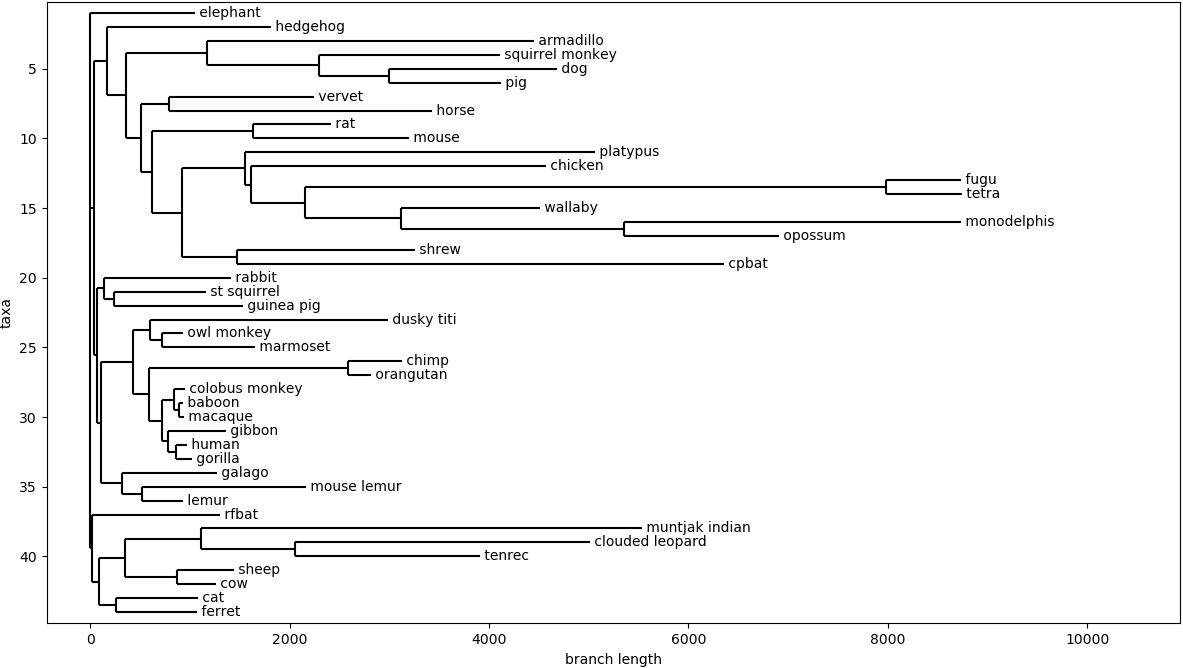
\includegraphics[width=\linewidth]{img/nj.png}
    \caption{The result of neighbor joining run on the coding dataset.}
    \label{fig:nj}
\end{figure*}

\begin{figure*}
    \centering
    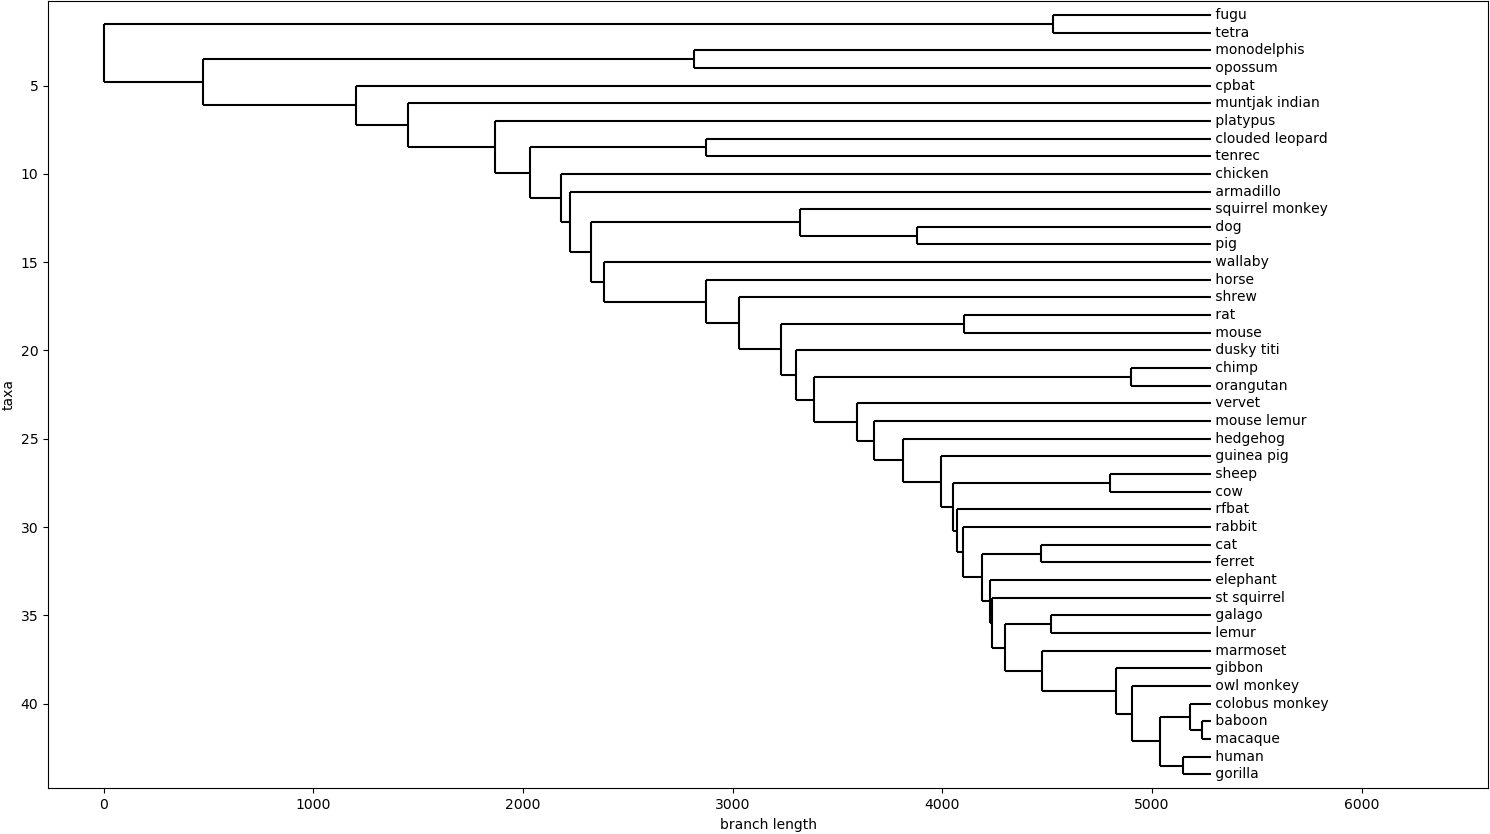
\includegraphics[width=\linewidth]{img/upgma.png}
    \caption{The result of UPGMA run on the coding dataset.}
    \label{fig:upgma}
\end{figure*}

\begin{figure*}
    \centering
    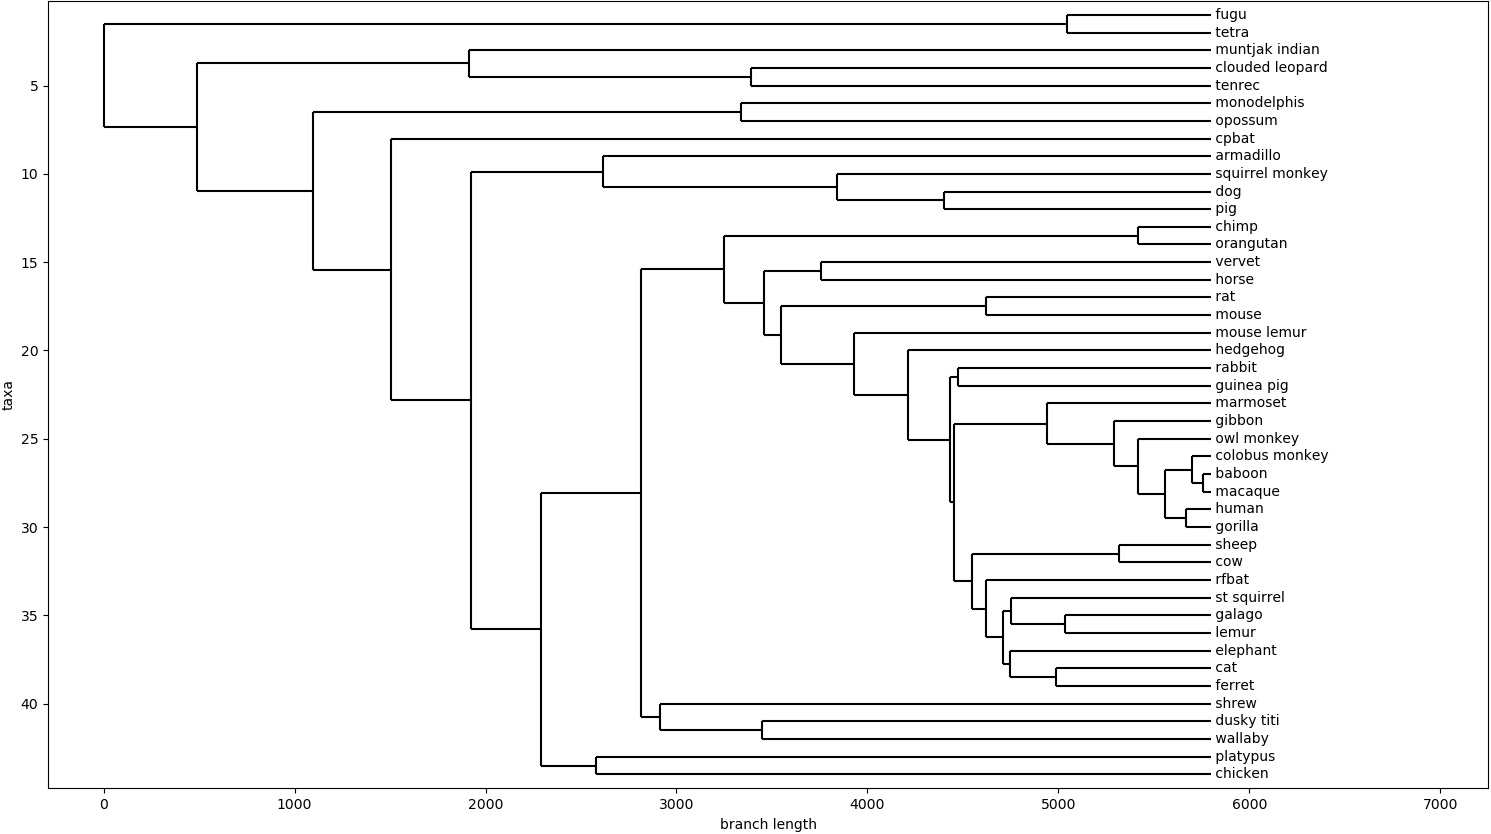
\includegraphics[width=\linewidth]{img/wpgma.png}
    \caption{The result of WPGMA run on the coding dataset.}
    \label{fig:wpgma}
\end{figure*}

\begin{figure*}
    \centering
    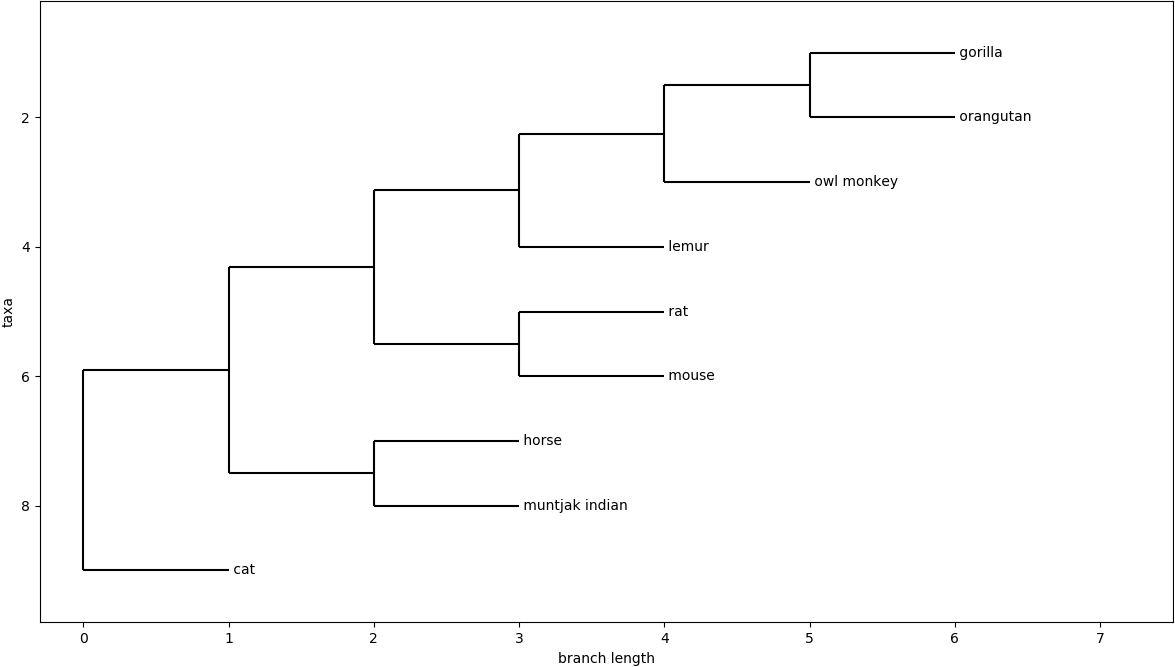
\includegraphics[width=\linewidth]{img/mp_9_taxa.png}
    \caption{The result of MP run on 9 elements of the coding dataset.}
    \label{fig:mp}
\end{figure*}

\begin{figure*}
    \centering
    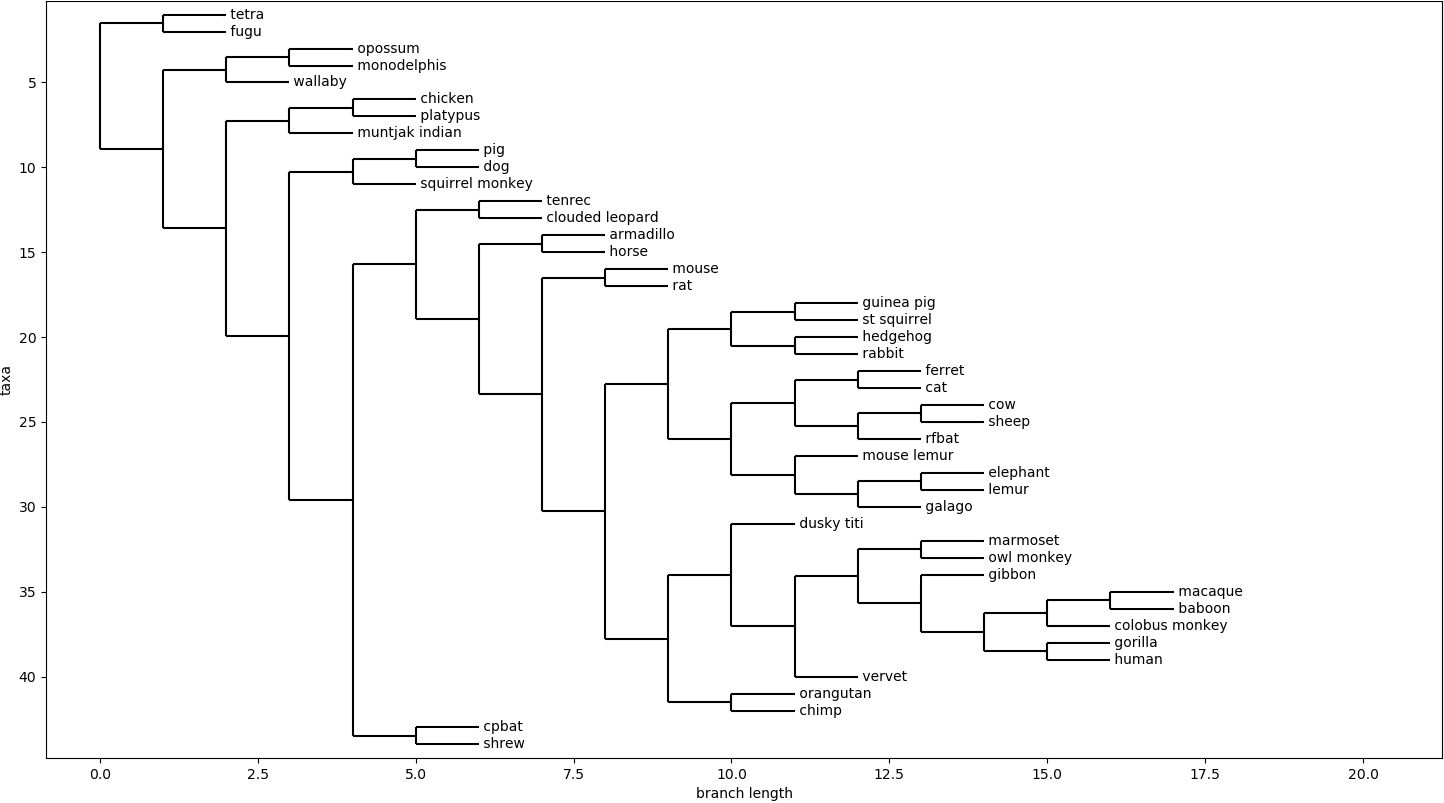
\includegraphics[width=\linewidth]{img/sota.png}
    \caption{The result of SOTA run on the coding dataset.}
    \label{fig:sota}
\end{figure*}

I first tested all five algorithms on the coding dataset. Regarding the result of neighbor joining (Figure \ref{fig:nj}), we can see that \textit{cats} and \textit{ferrets} are closely related (Carnivora, Laurasiatheria, Boreoeutheria), but they are further away from \textit{dogs} and \textit{pigs} which should be closely related to them according to the point of reference \cite{Prasad2008}. \textit{Sheep} and \textit{cows} are related (Cetartiodactyla), as well as species that are close to \textit{humans} (baboon, orangutan, chimp, gorilla, colobus monkey, macaque, gibbon). Neighbor joining managed to position other primates in the same cluster as well. The algorithm did well by placing some rodents in the vicinity of primates; it, however, put \textit{rats} and \textit{mice} into a different high-level category as humans. Other discrepancies include putting mostly dissimilar species like \textit{muntjak} and \textit{clouded leopard} next to each other but it can be said that it performed fairly well, especially since it is the most basic method.

When it comes to UPGMA (Figure \ref{fig:upgma}), cats and ferrets are still far from dogs and pigs but munjaks and leopards moved further from each other. Besides this, it performed a little worse than neighbor joining; \textit{chimps} and \textit{orangutans} have moved away from other primates, and other high-level categories remained mixed or obscure. Closely tied species still go together — \textit{tetraodon-fugu}, \textit{sheep-cow}, \textit{baboon-macaque}, \textit{rat-mouse}, \textit{human-gorilla} —, but other highly similar species — \textit{muntjak-cow}, \textit{horseshoe bat and short-tailed bat}, \textit{mouse lemur and right-tailed lemur}, \textit{owl money and squirrel monkey}, \textit{short-tailed opossum (monodelphis) and North American opossum (opossum)} — are separated from each other. It should be noted that the branch lengths are cascading because of the unweighted nature of this method.

In the case of WPGMA (Figure \ref{fig:wpgma}), only the mid-level clusters seem to have moved around compared to the structure of the tree produced by UPGMA. Most of the statements that apply to UPGMA are true of WPGMA as well. Slight improvements can be seen in certain relationships, e.g. \textit{platypuses} and \textit{chickens} got paired up and \textit{guinea pigs} got closer to \textit{rats} and \textit{mice}; these changes, however, are not sufficient to claim that there is a significant difference in UPGMA and WPGMA.

As mentioned before, time is an important factor when using maximum parsimony. The maximum number of taxa I ran the exact method on was 9, therefore only a subtree of the result is shown in Figure \ref{fig:mp}. The exact method has the capacity to evaluate every possible combination of branches, therefore the solution it provides is optimal. It can be said that the resulting tree bears a high degree of resemblance to Figure 1 in Prasad's paper \cite{Prasad2008}.

Finally, SOTA (Figure \ref{fig:sota})

\section{Conclusion}

Combining these methods by e.g. starting out from a tree pre-calculated with neighbor joining and then finding better solutions with maximum parsimony could result in a possible improvement in performance; such optimization techniques are often used in the field of phylogenetics \cite{Zvelebil2007}.

The repository is available on \href{https://github.com/Leena01/computational_biology}{GitHub}. Since the project provides a simplified overview of various phylogenetic methods, I hope that it can serve as reference for others who are interested in this field.

\bibliographystyle{unsrt}
\nocite{*}
\bibliography{report}

\end{document}
